\section{Invariants and Coinvariants of $ \mathfrak{g} $-modules} % (fold)
\label{sec:invariants}
Using the groundwork from the previous section we are now in a position to properly begin defining Lie algebra (co)homology and explore some fundamental results.

\subsection{Lie algebra (co)homology} % (fold)
\label{sub:Lie algebra (co)homology}
If $ V $ is a $ k $-module then there is a functor $ \text{triv}:k\text{-}\mathbf{Mod} \to \mathfrak{g}\text{-}\mathbf{Mod} $ which sends $ V $ to the trivial $ \mathfrak{g} $-module where $ xv = 0 $ for all $ x \in \mathfrak{g} $ and all $ v \in V $.

\begin{proposition}
  \label{prop:triv}
  The functor $ \text{triv} $ has a left adjoint, called the \textbf{coinvariant}, and a right adjoint, called the \textbf{invariant}.
\end{proposition}
\begin{proof}
  There are two canonical functors to consider:
  \begin{align*}
    &(-)_{\mathfrak{g}}: \mathfrak{g}\text{-}\mathbf{Mod} \to k\text{-}\mathbf{Mod}, \\
    &(-)^{\mathfrak{g}}: \mathfrak{g}\text{-}\mathbf{Mod} \to k\text{-}\mathbf{Mod},
  \end{align*}
  defined for $ M \in \mathfrak{g}\text{-}\mathbf{Mod} $ by
  \begin{align*}
    M_{\mathfrak{g}} &\coloneqq M/\mathfrak{g}M \\
    M^\mathfrak{g} &\coloneqq \{m \in M \mid xm=0 \text{ for all } x \in \mathfrak{g}\}
  .\end{align*}
  While the functor $ (-)^{\mathfrak{g}} $ simply takes $ \mathfrak{g} $-module homomorphisms to their restriction and considers them as $ k $-module homomorphisms, some remarks should be made about $ (-)_\mathfrak{g} $. Let therefore $ f: M \to N $ be a $ \mathfrak{g} $-module homomorphism and let $ \pi_N: N \to N_\mathfrak{g} $ be the projection $ k $-module homomorphism. We then have that $ \pi_N(f(\mathfrak{g}M)) = \pi_N(\mathfrak{g}f(M)) $ and so by the universal property of the quotient there exists a $ k $-module homomorphism $ f_\mathfrak{g}: M_\mathfrak{g} \to N_\mathfrak{g} $ such that $ \pi_N \circ f = f_\mathfrak{g}\circ \pi_M  $. It is fairly straightforward to see that this assignment is functorial and we leave the details of this to the reader.

  Our claim is that
  \begin{align*}
    (-)_{\mathfrak{g}} \dashv \text{triv} \dashv (-)^\mathfrak{g}
  .\end{align*}

  ($ (-)_{\mathfrak{g}} \dashv \text{triv} $): Let the unit
  \begin{equation}
    \eta: 1_{\mathfrak{g}\text{-}\mathbf{Mod}} \implies \text{triv}((-)_\mathfrak{g})
  \end{equation}
  be defined componentwise by the projection
  \begin{equation}
    \eta_M \coloneqq \pi_M : M \to \text{triv}(M_\mathfrak{g}).
  \end{equation}
  To see that $ \eta_M $ indeed is a $ \mathfrak{g} $-module homomorphism we must verify that the following diagram commutes
  \[\begin{tikzcd}
	  {\mathfrak{g} \otimes_kM} & {\mathfrak{g}\otimes_k\text{triv}(M_\mathfrak{g})} \\
	  M & {\text{triv}(M_\mathfrak{g})}
	  \arrow["0", from=1-2, to=2-2]
	  \arrow["{1_\mathfrak{g} \otimes \pi_M}", from=1-1, to=1-2]
	  \arrow[from=1-1, to=2-1]
	  \arrow["{\pi_M}"', from=2-1, to=2-2]
  \end{tikzcd}\]
  This is immediate as $ \pi_M(\mathfrak{g}M) = 0 $. Now, to verify naturality, let $ f: M \to N $ be a map of $ \mathfrak{g} $-modules. We want to check commutativity of the following diagram:
  \[\begin{tikzcd}
	  M & N \\
	  {\text{triv}(M_\mathfrak{g})} & {\text{triv}(N_\mathfrak{g}).}
	  \arrow["{\pi_M}"', from=1-1, to=2-1]
	  \arrow["f", from=1-1, to=1-2]
	  \arrow["{\text{triv}f_\mathfrak{g}}"', from=2-1, to=2-2]
	  \arrow["{\pi_N}", from=1-2, to=2-2]
  \end{tikzcd}\]
  This is immediate as given $ m \in M $ we have
  \begin{align*}
    \pi_N(f(m)) &= \overline{f(m)} \\
                &= f_\mathfrak{g}(\overline{m}) \\
                &= \text{triv}f_\mathfrak{g}(\overline{m})
  \end{align*}
  which shows commutativity.

  We define the counit
  \begin{equation}
    \epsilon:(\text{triv})_\mathfrak{g} \implies 1_{k\text{-}\mathbf{Mod}}
  \end{equation}
  componentwise as the identity. This is because $ (\text{triv}(V))_\mathfrak{g}=\text{triv}(V) $ and the underlying $ k $-module of $ \text{triv}(V) $ is just $ V $. Hence it make sense to define the counit componentwise as the identity:
  \begin{equation}
    \epsilon_V \coloneqq 1_V:(\text{triv}(V))_\mathfrak{g} \to V.
  \end{equation}
  Naturality then immediately follows as the identity transformation is natural.

  What remains to show then are the triangle identities:
  \begin{align*}
    \epsilon(-)_\mathfrak{g} \circ (-)_\mathfrak{g}\eta &= 1_{(-)_\mathfrak{g}} \\
    \text{triv}\,\epsilon \circ \eta\,\text{triv} &= 1_{\text{triv}}
  .\end{align*}
  Componentwise we have
  \begin{align*}
    \epsilon_{M_{\mathfrak{g}}} \circ (\eta_M)_\mathfrak{g} &= 1_{M_{\mathfrak{g}}} \circ (\pi_M)_\mathfrak{g} \\
                                                            &= (\pi_M)_\mathfrak{g} \\
                                                            &= 1_{M_\mathfrak{g}}
  \end{align*}
  and
  \begin{align*}
    \text{triv}(\epsilon_V) \circ \eta_{\text{triv}(V)} &= 1_{\text{triv}(V)} \circ \pi_{\text{triv}(V)} \\
                                                        &= \pi_{\text{triv}(V)} \\
                                                        &= 1_{\text{triv}(V)}
  \end{align*}
  where the last equality follows since $ (\text{triv}(V))_\mathfrak{g} = \text{triv}(V) $. Thus $ (-)_\mathfrak{g} \dashv \text{triv} $.


  ($ \text{triv} \dashv (-)^\mathfrak{g} $): As $ (-)^\mathfrak{g} \circ \text{triv} = 1_{k\text{-}\mathbf{Mod}} $ we can simply let the unit
  \begin{equation}
    \eta: 1_{k\text{-}\mathbf{Mod}} \implies (\text{triv})^\mathfrak{g}=1_{k\text{-}\mathbf{Mod}}
  \end{equation}
  be the identity. We then let the counit
  \begin{equation}
    \epsilon:  \text{triv}((-)^\mathfrak{g}) \implies 1_{g\text{-}\mathbf{Mod}}
  \end{equation}
  be the inclusion
  \begin{equation}
    \epsilon_M \coloneqq \iota_M:\text{triv}(M^\mathfrak{g}) \subset M.
  \end{equation}
  We must then verify the triangle identities
  \begin{align*}
    \epsilon\,\text{triv} \circ \text{triv}\,\eta &= 1_{\text{triv}} \\
    (-)^\mathfrak{g}\epsilon \circ \eta (-)^\mathfrak{g} &= 1_{(-)^\mathfrak{g}}
  .\end{align*}
  Componentwise we have
  \begin{align*}
    \epsilon_{\text{triv}(V)} \circ \text{triv}(\eta_V) &= \iota_{\text{triv}(V)} \circ \text{triv}(1_V) \\
                                                        &= \iota_{\text{triv}(V)} \circ 1_{\text{triv}(V)} \\
                                                        &= \iota_{\text{triv}(V)} \\
                                                        &= 1_{\text{triv}(V)}
  \end{align*}
  where the last equality follows because $ \text{triv}((\text{triv}(V))^\mathfrak{g}) = \text{triv}(V) $. We also have
  \begin{align*}
    (\epsilon_M)^\mathfrak{g} \circ \eta_{M^\mathfrak{g}} &= (\iota)^\mathfrak{g} \circ 1_{M^\mathfrak{g}} \\
                                                          &= (\iota_M)^\mathfrak{g} \\
                                                          &= 1_{M^\mathfrak{g}}
  \end{align*}
  where the last equality follows from the same reasoning as before. This then proves that $ \text{triv} \dashv (-)^\mathfrak{g} $.
\end{proof}

\begin{definition}[Lie algebra (co)homology]
  Let $ \mathfrak{g} $ be a Lie algebra and $ M $ a $ \mathfrak{g} $-module. The \textbf{homology groups of} $ \mathfrak{g} $ \textbf{with coefficients in} $ M $ is then defined as
  \begin{equation}
    H_*(\mathfrak{g}, M) \coloneqq L_*((-)_\mathfrak{g})(M)
  \end{equation}
  and the \textbf{cohomology groups of} $ \mathfrak{g} $ \textbf{with coefficients in} $ M $ is defined as
  \begin{equation}
    H^*(\mathfrak{g}, M) \coloneqq R^*((-)^\mathfrak{g})(M)
    \label{eq:cohomology}
  \end{equation}
  where $ L_* $ and $ R^* $ are the left and right derived functors respectively.
\end{definition}
The above definition of Lie algebra (co)homology in terms of derived functors is why it was so important to verify that $ \mathfrak{g} $-\textbf{Mod} was abelian and that it had enough projectives/injectives.

However, the definition above is quite impractical when it comes to actual computations and so it would be nice if we could relate it to something more concrete.
\begin{proposition}
  \label{prop:torext}
  Let $ \mathfrak{g} $ be a Lie algebra and $ M $ a $ \mathfrak{g} $-module. We then have
  \begin{align*}
    H_*(\mathfrak{g}, M) &\cong \text{Tor}^{U\mathfrak{g}}_*(k, M) \\
    H^*(\mathfrak{g}, M) &\cong \text{Ext}^*_{U\mathfrak{g}}(k, M)
  .\end{align*}
\end{proposition}
\begin{proof}
  Following the argumentation in Corollary 7.3.6 of \cite{weibel1994homological} we note that two derived functors are isomorphic whenever the underlying functors are isomorphic. Now, as
  \begin{align*}
    H_*(\mathfrak{g}, M) &= L_*((-)_\mathfrak{g})(M) \\
    \text{Tor}_*^{U\mathfrak{g}}(k, M) &= L_*(k \otimes_{U\mathfrak{g}} -)(M)
  \end{align*}
  we need to prove that $ (-)_\mathfrak{g} \cong k \otimes_{U\mathfrak{g}} - $. To this end, let $ \epsilon: U\mathfrak{g} \to k $ be the augmentation of $ k $ which sends $ i(\mathfrak{g})U\mathfrak{g} $ to zero and $ k $ to itself. The kernel of $ \epsilon $ is then generated by $ \iota_\mathfrak{g}(\mathfrak{g}) $ where $ i: \mathfrak{g} \to U\mathfrak{g} $ is the inclusion of $ \mathfrak{g} $ into $ U\mathfrak{g} $. Denoting $ \text{ker}(\epsilon) $ by $ \mathfrak{J} $ we therefore have that $ \mathfrak{J} $ is a $ U\mathfrak{g} $-module. Moreover
  \begin{equation}
    M/\mathfrak{J}M \cong \mathfrak{g}M
  \end{equation}
  which follows as the action of any $ \overline{x} \in \mathfrak{J} $ on $ M $ can be reduced to an action of some $ x \in \mathfrak{g} $ on $ M $.
  Thus
  \begin{align*}
    k \otimes_{U\mathfrak{g}} M &\cong (U\mathfrak{g}/\mathfrak{J}) \otimes_{U\mathfrak{g}} M \\
  &\cong M/\mathfrak{J}M \\
  &\cong M/\mathfrak{g}M \\
  &\cong M_\mathfrak{g}
\end{align*}
showing that the two underlying functors are the same.

Similarly, for cohomology, we want to show that the two functors $ (-)^\mathfrak{g} $ and $ \text{Hom}_{U\mathfrak{g}}(k, -) $ are isomorphic. To see this note first that $ M^\mathfrak{g} \cong \text{Hom}_{\mathfrak{g}\text{-}\mathbf{Mod}}(k, M) $ when considering $ k $ as a trivial $ \mathfrak{g} $-module. From this and Proposition~\ref{prop:gmodeq} it follows that
\begin{equation}
  \text{Hom}_{U\mathfrak{g}}(k, M) \cong \text{Hom}_{\mathfrak{g}\text{-}\mathbf{Mod}}(k, M) \cong M^{\mathfrak{g}}
  \label{eq:cohomsame}
\end{equation}
which proves the claim.
\end{proof}

Having the Lie algebra (co)homology defined in terms of Ext and Tor will allow to show some rudimentary results. For one of these results we need a little lemma.
\begin{lemma}
  Let $ \epsilon: U\mathfrak{g} \to \mathfrak{g} $ be the augmentation map and $ \mathfrak{J} $ the kernel of this map. We then have that
  \begin{equation}
    \mathfrak{J}/\mathfrak{J}^2 \cong \mathfrak{g}/[\mathfrak{g}, \mathfrak{g}]
    \label{eq:abelianization}
  \end{equation}
  as $ k $-modules.
\end{lemma}
\begin{proof}
  This is a solution to \cite[Exercise 7.4.1]{weibel1994homological}.

  Let $ \{e_\alpha\} $ be a ordered basis for $ \mathfrak{g} $ and consider the map $ i: \mathfrak{g} \to U\mathfrak{g} $. We have that
  \begin{equation}
    i([e_{\alpha},e_{\beta}]) = e_{(\alpha, \beta)} - e_{(\beta, \alpha)}.
  \end{equation}
  Moreover
  \begin{equation}
    e_{(\alpha,\beta)} - e_{(\beta, \alpha)} = e_{(\alpha)}e_{(\beta)} - e_{(\beta)}e_{(\alpha)} \in \mathfrak{J}^2
  \end{equation}
  meaning that $ i $ induces a map $ i':\mathfrak{g}/[\mathfrak{g}, \mathfrak{g}] \to \mathfrak{J}/\mathfrak{J}^2 $. We then just need to find a $ k $-module homomorphism $ \sigma': \mathfrak{J} \to \mathfrak{g}/[\mathfrak{g}, \mathfrak{g}] $ which is an inverse to $ i' $ when taking the quotient of $ \mathfrak{J} $ with $ \mathfrak{J}^2 $. We define it on basis elements as follows:
  \begin{equation}
    \sigma'(e_{(\alpha_1, \ldots, \alpha_n)}) = \begin{cases}
      0, &\text{ if } n \geq 2, \\
      \overline{e}_{\alpha_1} &\text{ else.}
    \end{cases}
  \end{equation}
  Since $ \sigma'(\mathfrak{J}^2) = 0 $ we have a unique $ k $-module homomorphism $ \sigma: \mathfrak{J}/\mathfrak{J}^2 \to \mathfrak{g}/[\mathfrak{g}, \mathfrak{g}] $ such that $ \sigma' = \sigma \circ \pi $ where $ \pi: \mathfrak{J} \to \mathfrak{J}/\mathfrak{J}^2 $ is the quotient map. Our claim is that $ \sigma $ is an inverse to $ i' $. To see this, let $ \overline{e}_\alpha \in \mathfrak{g}/[\mathfrak{g}, \mathfrak{g}] $ be a generator of this quotient module. We then have that
  \begin{align*}
    (\sigma \circ i')(\overline{e}_\alpha) &= \sigma(i'(\overline{e}_\alpha)) \\
                                           &= \sigma(\overline{i(e_\alpha)}) \\
                                           &= \sigma(\overline{e}_{(\alpha)}) \\
                                           &= \overline{\sigma(e_{(\alpha)})} \\
                                           &= \overline{e}_\alpha
  \end{align*}
  and hence $ \sigma \circ i' = 1_{\mathfrak{g}/[\mathfrak{g}, \mathfrak{g}]} $. Next, let $ \overline{e}_{(\alpha)} $ be a generator of $ \mathfrak{J}/\mathfrak{J}^2 $. We then have
  \begin{align*}
    (i' \circ \sigma)(\overline{e}_{\alpha}) &= i'(\sigma(\overline{e}_{(\alpha)})) \\
                                             &= i'(\overline{\sigma(e_{(\alpha)})}) \\
                                             &= i'(\overline{e}_{\alpha}) \\
                                             &= \overline{i(e_{\alpha})} \\
                                             &= \overline{e}_{(\alpha)}
  \end{align*}
  showing that $ \sigma \circ i' = 1_{\mathfrak{J}/\mathfrak{J}^2} $ as well. Hence $ i' $ and $ \sigma $ are mutual $ k $-module inverses, completing the proof.
\end{proof}


\begin{corollary}
  \label{cor:abelianization}
  If $ M $ is a trivial $ \mathfrak{g} $-module then
  \begin{equation}
    H_1(\mathfrak{g}, M) \cong (\mathfrak{g}/[\mathfrak{g}, \mathfrak{g}]) \otimes_k M.
  \end{equation}
\end{corollary}
\begin{proof}
  The following is an adaptation of \cite[Corollary 7.3.6]{weibel1994homological}.
  Since $ U\mathfrak{g} $ is a projective $ U\mathfrak{g} $-module we have that $ \text{Tor}_1^{U\mathfrak{g}}(U\mathfrak{g}, M) = 0 $. We have a short exact sequence
  \begin{equation}
    0 \to \mathfrak{J} \xrightarrow{\iota} U\mathfrak{g} \xrightarrow{\epsilon} k \to 0
  \end{equation}
  with $ \iota $ being the inclusion and $ \epsilon $ the augmentation. Now, as $ U\mathfrak{g} $ is projective, we have that $ \text{Tor}_{1}^{U\mathfrak{g}}(U\mathfrak{g}, M) = 0 $ and hence the associated long exact sequence has the form:
  \begin{equation}
    0 \to \text{Tor}_1^{U\mathfrak{g}}(\mathfrak{g}, M) \to \text{Tor}_0^{U\mathfrak{g}}(\mathfrak{J}, M) \to \text{Tor}_0^{U\mathfrak{g}}(U\mathfrak{g}, M) \to \text{Tor}_0^{U\mathfrak{g}}(k, M) \to 0
  \end{equation}
  which is equivalent to the exact sequence
  \begin{equation}
    0 \to H_1(\mathfrak{g}, M) \to \mathfrak{J} \otimes_{U\mathfrak{g}} M \to M \to M_{\mathfrak{g}} \to 0.
  \end{equation}
  Since $ M $ is a trivial $ \mathfrak{g} $-module we have that $ M_\mathfrak{g} = M $ so that the second rightmost map is an isomorphism. From this it follows that
  \begin{equation}
    H_1(\mathfrak{g}, M) \cong \mathfrak{J} \otimes_{U\mathfrak{g}} M.
  \end{equation}
  Now, as
  \begin{align*}
    \mathfrak{J} \otimes_{U\mathfrak{g}} k &\cong \mathfrak{J} \otimes_{U\mathfrak{g}} (U\mathfrak{g}/\mathfrak{J}) \\
                                           &\cong \mathfrak{J}/\mathfrak{J}^2 \\
                                           &\cong \mathfrak{g}/[\mathfrak{g}, \mathfrak{g}]
  \end{align*}
  we have
  \begin{align*}
    \mathfrak{J} \otimes_{U\mathfrak{g}} M &\cong (J \otimes_{U\mathfrak{g}} k) \otimes_k M \\
                                           &\cong (\mathfrak{g}/[\mathfrak{g}, \mathfrak{g}]) \otimes_k M
  \end{align*}
  and so $ H_1(\mathfrak{g}, M) \cong \mathfrak{J} \otimes_{U\mathfrak{g}} M \cong \left( \mathfrak{g}/[\mathfrak{g}, \mathfrak{g}] \right) \otimes_k M $ as desired.
\end{proof}
% subsection Lie algebra (co)homology (end)

\subsection{The Chevalley-Eilenberg Complex} % (fold)
\label{sub:The Chevalley-Eilenberg Complex}
Although Proposition~\ref{prop:torext} is more helpful for showing results pertaining to Lie algebra (co)homology than our original definition using derived functors, it offers no insight into the construction of a projective resolution, which is essential for computing the (co)homology. To find such a projective resolution we must start with defining the exterior product.

\begin{definition}[Exterior algebra]
  Let $ M $ be a $ k $-module and $ I $ the ideal of $ T(M) $ generated by elements of the form $ x \otimes x $ for $ x \in M $. The \textbf{exterior algebra} of $ M $, denoted by $ \Lambda M $, is the quotient of $ T(M) $ with $ I $, i.e.,
  \begin{equation}
    \Lambda M\coloneqq T(M)/I.
  \end{equation}
  We let $ x_1 \wedge \cdots \wedge x_n $ denote the equivalence class of $ x_1 \otimes \cdots \otimes x_n $. Note that if $ k $ is a field then $ \Lambda M $ is free with basis $ x_1 \wedge \cdots \wedge x_n $ for $ n\geq 0 $ ($ n = 0 $ is the empty wedge product which is just the unit $ 1 \in k $).

  The $ n $\textbf{th exterior product of} $ M $, denoted $ \Lambda^{n}M $ is defined to be the submodule of $ \Lambda M $ spanned by elements of the form $ x_1 \wedge \cdots \wedge x_n $.
\end{definition}
To make life easier for ourselves later we will use the following notation
\begin{equation}
  \wedge(x_1, \widehat{x}_{i_1}, \cdots, \widehat{x}_{i_k}, x_n) =  x_1 \wedge \cdots \wedge x_{i_1 - 1} \wedge \widehat{x}_{i_1} \wedge x_{i_1 + 1} \wedge \cdots x_{i_k - 1} \wedge \widehat{x}_{i_{k}} \wedge x_{i_{k} + 1} \wedge \cdots \wedge x_{n}
\end{equation}
where $ (i_1, \ldots, i_k) $ is an increasing sequence and the notation $ \widehat{x}_i $ indicates that $ x_i $ is removed from the wedge product. Moreover if $ \{e_{\beta}\} $ is a basis for the Lie algebra $ \mathfrak{g} $ over $ k $ and $ J = (\beta_1, \ldots, \beta_n) $ is a strictly increasing sequence---meaning $ \beta_1 < \cdots < \beta_n $---then we will use the notation
\begin{equation}
  e^{J} = e_{\alpha_1} \wedge \cdots \wedge e_{\alpha_n}
\end{equation}
to denote the wedge product of basis elements where, again, the empty sequence $ \phi = () $ gives the unit $ e^{\phi} = 1 \in k $.

\begin{definition}[Chevalley-Eilenberg complex]
  Let $ \mathfrak{g} $ be a Lie algebra over $ k $ with basis set $ \{e_{\alpha}\} $. The $ n $th component of the \textbf{Chevalley-Eilenberg complex} is then defined to be
  \begin{equation}
    V_n(\mathfrak{g}) \coloneqq U\mathfrak{g} \otimes_k \Lambda^{n} \mathfrak{g}.
    \label{eq:cheval}
  \end{equation}
  As $ \Lambda \mathfrak{g} $ is free, when considered as a $ k $-module, it follows that $ V_n(\mathfrak{g}) $ is a free $ U\mathfrak{g} $-module. From Equation~\ref{eq:cheval} it follows that
  \begin{align*}
    V_1(\mathfrak{g}) &= U\mathfrak{g} \otimes_k \mathfrak{g} \\
    V_0(\mathfrak{g}) &= U\mathfrak{g} \otimes_k k \cong U\mathfrak{g}
  .\end{align*}
  We therefore define the map $ d_1: V_1(\mathfrak{g}) \to V_0(\mathfrak{g}) $ as multiplication, i.e., for basis elements $ e_I $ and $ e^{(\beta)} $ we have
  \begin{equation}
    d_1(e_I \otimes e^{(\beta)}) = e_I e_{(\beta)}.
  \end{equation}
  For $ n\geq 2 $ we let $ d_n $ be given on basis elements $ e_I $ and $ e^J $, where $ I = (\alpha_1, \ldots, \alpha_k) $ and $ J = (\beta_1, \ldots, \beta_n) $, by
  \begin{equation}
    d_n(e_I \otimes e^J) = \theta_1 + \theta_2
  \end{equation}
  where
  \begin{align*}
    \theta_1 &= \sum_{i = 1}^{n} (-1)^{n + 1}e_{(I, \beta_i)} \otimes \wedge(e_{\beta_1}, \widehat{e}_{\beta_i}, e_{\beta_n}) \\
    \theta_2 &= \sum_{i < j} (-1)^{i + j}e_I \otimes [e_{\beta_i}, e_{\beta_j}] \wedge(e_{\beta_1}, \widehat{e}_{\beta_i}, \widehat{e}_{\beta_j}, e_{\beta_n})
  \end{align*}
  where we abuse notation slightly so that $ e_{(I, \beta_i)} = e_{I}e_{(\beta_i)} $ and $ [e_{\beta_i}, e_{\beta_j}]\wedge (e_{\beta_1}, \widehat{e}_{\beta_i}, \widehat{e}_{\beta_j}, e_{\beta_n}) = [e_{\beta_i}, e_{\beta_j}]\wedge(\wedge(e_{\beta_1}, \widehat{e}_{\beta_i}, \widehat{e}_{\beta_j}, e_{\beta_n})) $.
\end{definition}

The above definition inherently contains the claim that $ d^2 = 0 $.
\begin{claim}
  The Chevalley-Eilenberg complex $ (V_*(\mathfrak{g}), d_*) $ is a chain complex.
\end{claim}
\begin{proof}
  We must show that $ d^2 = 0 $. Let $ \{e_{\alpha}\} $ be a basis for $ \mathfrak{g} $ and $ I = (\alpha_1, \ldots, \alpha_k) $ and $ J = (\beta_1, \ldots, \beta_n) $ an increasing and strictly increasing sequence, respectively. We then have that
  \begin{align*}
    d_{n - 1}(d_n(e_I \otimes e^J)) &= d_{n - 1}(\theta_1) + d_{n-1}(\theta_2) \\
                                    &= \theta_{11} + \theta_{12} + \theta_{21} + \theta_{22}
  \end{align*}
  where $ \theta_{i1} $ is the first part of $ d(\theta_i) $ and $ \theta_{i2} $ is the second part of $ d(\theta_{i}) $ and where $ i = 1,2 $. Expanding this we have that
  \begin{align*}
    \theta_{11} = &\sum_{r < i} (-1)^{i + r} e_{(I, \beta_i, \beta_r)} \otimes \wedge(e_{\beta_1}, \widehat{e}_{\beta_r}, \widehat{e}_{\beta_i}, e_{\beta_n}) \\
    + &\sum_{i < r} (-1)^{i + r + 1} e_{(I, \beta_i, \beta_r)} \otimes \wedge(e_{\beta_1}, \widehat{e}_{\beta_i}, \widehat{e}_{\beta_{r}}, e_{\beta_n}) \\
    \\
    \theta_{12} = &\sum_{r < s < i} (-1)^{i + r + s + 1} e_{(I, \beta_i)} \otimes [e_{\beta_r}, e_{\beta_s}] \wedge (e_{\beta_1}, \widehat{e}_{\beta_r}, \widehat{e}_{\beta_s}, \widehat{e}_{\beta_i}, e_{\beta_n}) \\
                  +&\sum_{r < i < s} (-1)^{i + r + s} e_{(I, \beta_i)} \otimes [e_{\beta_r}, e_{\beta_s}] \wedge (e_{\beta_1}, \widehat{e}_{\beta_r}, \widehat{e}_{\beta_i}, \widehat{e}_{\beta_s}, e_{\beta_n}) \\
                  +&\sum_{i < r < s} (-1)^{i + r + s + 1} e_{(I, \beta_i)} \otimes [e_{\beta_r}, e_{\beta_s}] \wedge (e_{\beta_1}, \widehat{e}_{\beta_i}, \widehat{e}_{\beta_r}, \widehat{e}_{\beta_s}, e_{\beta_n}) \\
                  \\
  \theta_{21} = & \sum_{i < j} (-1)^{i + j} (e_{(I, \beta_i, \beta_j)} - e_{(I, \beta_j, \beta_i)}) \otimes \wedge(e_{\beta_1}, \widehat{e}_{\beta_i}, \widehat{e}_{\beta_j}, e_{\beta_n}) \\
  +& \sum_{r < i < j} (-1)^{i + j + r}e_{(I, \beta_r)} \otimes [e_{\beta_i}, e_{\beta_j}] \wedge(e_{\beta_1}, \widehat{e}_{\beta_r}, \widehat{e}_{\beta_i}, \widehat{e}_{\beta_j}, e_{\beta_n}) \\
  +& \sum_{i < r < j} (-1)^{i + j + r + 1}e_{(I, \beta_r)} \otimes [e_{\beta_i}, e_{\beta_j}] \wedge(e_{\beta_1}, \widehat{e}_{\beta_i}, \widehat{e}_{\beta_r}, \widehat{e}_{\beta_j}, e_{\beta_n}) \\
  +&\sum_{i < j < r} (-1)^{i + j + r}e_{(I, \beta_r)} \otimes [e_{\beta_i}, e_{\beta_j}] \wedge(e_{\beta_1}, \widehat{e}_{\beta_i}, \widehat{e}_{\beta_j}, \widehat{e}_{\beta_r}, e_{\beta_n}) \\
  \\
  \theta_{22} = &\sum_{s < i < j}(-1)^{i + j + s} e_{I} \otimes \left[[x_i, x_j], x_s \right] \wedge(e_{\beta_1}, \widehat{e}_{\beta_s}, \widehat{e}_{\beta_i}, \widehat{e}_{\beta_j}, e_{\beta_n}) \\
  +&\sum_{i < s < j}(-1)^{i + j + s + 1} e_{I} \otimes \left[[x_i, x_j], x_s \right] \wedge(e_{\beta_1}, \widehat{e}_{\beta_i}, \widehat{e}_{\beta_s}, \widehat{e}_{\beta_j}, e_{\beta_n}) \\
  +&\sum_{i < j < s}(-1)^{i + j + s} e_{I} \otimes \left[[x_i, x_j], x_s \right] \wedge(e_{\beta_1}, \widehat{e}_{\beta_i}, \widehat{e}_{\beta_j}, \widehat{e}_{\beta_s}, e_{\beta_n}) \\
  +&\sum_{r < s <i < j }(-1)^{i + j + r + s} e_{I} \otimes [x_r, x_s] \wedge [x_i, x_j]  \wedge(e_{\beta_1}, \widehat{e}_{\beta_r}, \widehat{e}_{\beta_s}, \widehat{e}_{\beta_i}, \widehat{e}_{\beta_j}, e_{\beta_n}) \\
  +&\sum_{r < i < s < j }(-1)^{i + j + r + s + 1} e_{I} \otimes [x_r, x_s] \wedge [x_i, x_j]  \wedge(e_{\beta_1}, \widehat{e}_{\beta_r}, \widehat{e}_{\beta_i}, \widehat{e}_{\beta_s}, \widehat{e}_{\beta_j}, e_{\beta_n}) \\
  +&\sum_{r < i <j < s }(-1)^{i + j + r + s} e_{I} \otimes [x_r, x_s] \wedge [x_i, x_j]  \wedge(e_{\beta_1}, \widehat{e}_{\beta_r}, \widehat{e}_{\beta_i}, \widehat{e}_{\beta_j}, \widehat{e}_{\beta_s}, e_{\beta_n}) \\
  +&\sum_{i < r <s < j }(-1)^{i + j + r + s} e_{I} \otimes [x_r, x_s] \wedge [x_i, x_j]  \wedge(e_{\beta_1}, \widehat{e}_{\beta_i}, \widehat{e}_{\beta_r}, \widehat{e}_{\beta_s}, \widehat{e}_{\beta_j}, e_{\beta_n}) \\
  +&\sum_{i < r <j < s }(-1)^{i + j + r + s + 1} e_{I} \otimes [x_r, x_s] \wedge [x_i, x_j]  \wedge(e_{\beta_1}, \widehat{e}_{\beta_i}, \widehat{e}_{\beta_r}, \widehat{e}_{\beta_j}, \widehat{e}_{\beta_r}, e_{\beta_n}) \\
  +&\sum_{i < j <r < s }(-1)^{i + j + r + s} e_{I} \otimes [x_r, x_s] \wedge [x_i, x_j]  \wedge(e_{\beta_1}, \widehat{e}_{\beta_i}, \widehat{e}_{\beta_j}, \widehat{e}_{\beta_i}, \widehat{e}_{\beta_j}, e_{\beta_n}).
  \end{align*}
  From this we see that $ \theta_{11} $ cancels out the 1st sum in $ \theta_{21} $. We then see that the 1st sum in $ \theta_{12} $ cancels out the 4th sum in $ \theta_{21} $, the 2nd sum in $ \theta_{12} $ cancels out the 3rd sum in $ \theta_{21} $, and the 3rd sum in $ \theta_{12} $ cancels out the 2nd sum in $ \theta_{21} $, which together means that
  \begin{equation}
    \theta_{11} + \theta_{12} + \theta_{21} = 0.
  \end{equation}
  Next, in $ \theta_{22} $ the 1st and 3rd sum cancel out the 2nd sum (by the Jacobi identity), the 4th sum cancels out the 9th sum, the 5th sum cancels out the 8th sum, and the 6th sum cancels out the 7th sum, which all together means that $ \theta_{22} = 0 $. Hence
  \begin{equation}
    \theta_{11} + \theta_{12} + \theta_{21} + \theta_{22} = 0
  \end{equation}
  which means that $ d^2 = 0 $ as desired.
\end{proof}

More can be said about the Chevalley-Eilenberg complex as it gives us a concrete way to compute Lie algebra (co)homology.
\begin{theorem}
  \label{thm:cheval}
  The Chevalley-Eilenberg complex $ (V_{*}(\mathfrak{g}), d_*) $ together with the augmentation map $ \epsilon: U\mathfrak{g} \to k $ gives a projective resolution $ V_*(\mathfrak{g})\xrightarrow{\epsilon} k $ of $ k $ as a trivial $ \mathfrak{g} $-module.
\end{theorem}
\begin{proof}
  We follow the outline presented in the proof of Theorem 1.3.1 in \cite{Jansen2016LieAlgebraCohomology}.

  Our goal is to prove exactness of the following complex
  \[\begin{tikzcd}
	  \cdots & {U\mathfrak{g} \otimes_k \Lambda^2\mathfrak{g}} & {U\mathfrak{g} \otimes_k\mathfrak{g}} & {U\mathfrak{g}} & k & 0.
	  \arrow["{d_3}", from=1-1, to=1-2]
	  \arrow["{d_2}", from=1-2, to=1-3]
	  \arrow["{d_1}", from=1-3, to=1-4]
	  \arrow["\varepsilon", from=1-4, to=1-5]
	  \arrow[from=1-5, to=1-6]
  \end{tikzcd}\]

  Now, to see that the Chevalley-Eilenberg complex has trivial homology we start by fixing some notation. Let $ U^{k}\mathfrak{g} $ be the image of $ \bigoplus_{i = 0}^{k} \mathfrak{g}^{\otimes i} \subset T(\mathfrak{g}) $ in $ U\mathfrak{g} $. We then define a filtration $ F $ of $ V_*(\mathfrak{g}) $ as follows
  \begin{equation}
    F_{p, n} = \begin{cases}
      U^{p - n}\mathfrak{g} \otimes_k \Lambda^{n} \mathfrak{g}, &\text{ if } n \leq p,\\
      k, &\text{ if }  n = -1 ,\\
      0, &\text{ else.}
    \end{cases}
  \end{equation}
  \begin{figure}[t]
    \begin{center}
      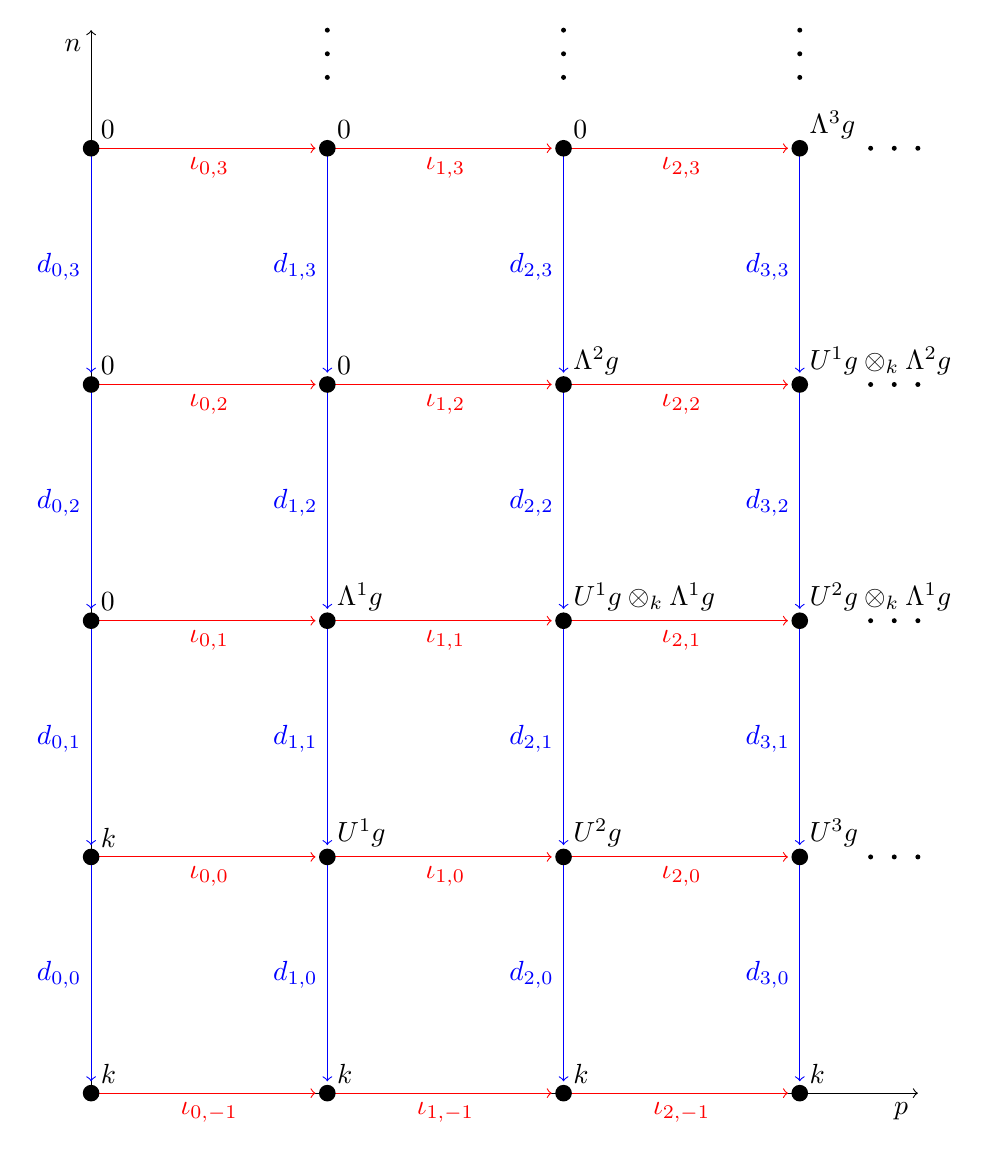
\begin{tikzpicture}[scale=3]  % Increased scale for better visibility
        % Grid dimensions
        \def\maxn{3} % Adjust as needed
        \def\minn{-1} % New minimum n value
        \def\maxp{3} % Adjust as needed

        % Drawing the axes
        \draw[->] (0,-1) -- (\maxp+0.5,-1) node[anchor=north east] {$p$};
        \draw[->] (0,-1) -- (0,\maxn+0.5) node[anchor=north east] {$n$};

        % Drawing the lattice points, labels, and differential maps
        \foreach \n in {\minn,...,\maxn} {
          \foreach \p in {0,...,\maxp} {
            % Calculate p - n
            \pgfmathtruncatemacro{\diff}{\p - \n}

            % Conditional structure for labeling
            \ifnum\n=-1
              \node[anchor=south west, black] at (\p,\n) {$k$}; % Special row for n = -1
            \else
              \ifnum\n>\p
                \node[anchor=south west, black] at (\p,\n) {0}; % Label as zero if n > p
              \else
                \ifnum\n=\p
                  \ifnum\n=0 % Special case for M_{0,0} = k
                    \node[anchor=south west, black] at (\p,\n) {$k$};
                  \else % Special case for diagonal (Lambda^n g)
                    \node[anchor=south west, black] at (\p,\n) {$\Lambda^\n \mathfrak{g}$};
                  \fi
                \else
                  \ifnum\n=0 % Special case for p-axis (p > 0, n = 0)
                    \node[anchor=south west, black] at (\p,\n) {$U^{\p}\mathfrak{g}$};
                  \else % General case
                    \node[anchor=south west, black] at (\p,\n) {$U^{\diff}\mathfrak{g} \otimes_k \Lambda^\n \mathfrak{g}$};
                  \fi
                \fi
              \fi
            \fi

            % Draw differential maps (vertical arrows)
            \ifnum\n>-1
              \draw[->, blue] (\p,\n) -- (\p,\n-0.95); % Vertical differential
              \node[anchor=east, blue] at (\p,\n-0.5) {$d_{\p,\n}$};
            \fi
            \ifnum\p<\maxp
              \draw[->, red] (\p,\n) -- (\p+0.95,\n); % Horizontal inclusion
              \node[anchor=north, red] at (\p+0.5,\n) {$\iota_{\p,\n}$};
            \fi


            % Draw lattice points
            \fill (\p,\n) circle (1pt);

          }
        }

        % Adding dots to indicate continuation
        \foreach \n in {0,...,\maxn} {
          \fill (\maxp+0.3,\n) circle (0.3pt);  % Dots on the right side
          \fill (\maxp+0.4,\n) circle (0.3pt);
          \fill (\maxp+0.5,\n) circle (0.3pt);
        }
        \foreach \p in {1,...,\maxp} {
          \fill (\p,\maxn+0.3) circle (0.3pt);  % Dots on the top side
          \fill (\p,\maxn+0.4) circle (0.3pt);
          \fill (\p,\maxn+0.5) circle (0.3pt);
        }
      \end{tikzpicture}
    \end{center}
    \caption{A small portion of $ F_{p, n} $ for $ -1 \leq n \leq 3 $ and $ 0 \leq p \leq 3 $ where the blue arrows are the induced differential maps on $ F_p $ and the red arrows are the inclusion maps. Notice that $ F_p $ is the sum of the $ F_{p,n} $'s along the vertical.}\label{fig:filtrationf}
  \end{figure}
  The filtration can be visualized on a 2d lattices as shown in Figure~\ref{fig:filtrationf}. Note that we define the maps $ d_{p, 0}:F_{p, 0} \to F_{p, -1} $ to be the restriction of the augmentation map, i.e., $ d_{p, 0} = \epsilon|_{U^{p}\mathfrak{g}} $. Moreover, for $ n>0 $ we let $ d_{p, n}: F_{p, n} \to F_{p, n-1} $ be the restriction of $ d_n $ to $ F_{p,n} $ and as $ d_n(F_{p, n}) \subset F_{p, n-1} $ we have a well defined boundary map which squares to zero and hence makes $ F_p $ into a chain complex.

  For $ n\geq 0 $ the inclusion $\iota'_{k-1}: U^{k-1}\mathfrak{g} \to U^{k}\mathfrak{g} $ extends to an inclusion $ \iota_{p, n}: F_{p, n} \to F_{p+1, n} $ which is natural with respect to the boundary map $ d_{p, n} $ (we set $ \iota_{-1, p} $ to be the identity on $ k $). We thus have an induced map of chain complexes $ \iota_p: F_p \to F_{p + 1} $. This gives rice to a sequence of inclusions $ F_0 \subset F_1 \subset \cdots \subset F_p \subset \cdots $ with direct limit equal to $ \bigcup_{p = 0}^{\infty} F_p = V_{*}(\mathfrak{g}) \xrightarrow{\epsilon} k $. As homology preserves direct limits we then have that
  \begin{align*}
    H_*\left( V_{*}(\mathfrak{g}) \xrightarrow{\epsilon} k\right) &= H_* \left( \bigcup_{p = 0}^{\infty} F_p \right) \\
                                                                  &= H_* \left( \varinjlim{F_p} \right) \\
                                                                  &= \varinjlim{H_*(F_p)}
  \end{align*}
  and so if we can show that $ H_*(F_p) = 0 $ then we are done.

  To this end, for $ p \geq 1 $ we define a new chain complex $ W_p = \text{coker}(\iota_{p - 1}) $ which more explicitly is given by
  \begin{equation}
    W_{p, n} = \begin{cases}
      F_{p, n}/F_{p-1, n}, &\text{ if } n \geq 0,\\
      0, &\text{ else}.
    \end{cases}
  \end{equation}

  This gives us a short exact sequence of chain complexes:
  \begin{equation}
    \label{eq:ses}
    0 \to F_{p - 1} \xrightarrow{\iota} F_p \xrightarrow{\pi} W_p \to 0.
  \end{equation}
  Note that, since $ \Lambda^{n}\mathfrak{g} $ is a free $ k $-module, tensoring with $ \Lambda^{n}\mathfrak{g} $ preserves exactness and so for $ 0\leq n \leq p $ we have
  \begin{equation}
    W_{p, n} = (U^{p - n}\mathfrak{g}\otimes_k \Lambda^{n}\mathfrak{g}) /(U^{p - n - 1}\mathfrak{g}\otimes_k \Lambda^{n}\mathfrak{g}) \cong (U^{p - n}\mathfrak{g} /U^{p - n - 1}\mathfrak{g})\otimes_k \Lambda^{n}\mathfrak{g}.
  \end{equation}

  We can visualize the modules $ W_{p, n} $ on a 2d lattice as done in Figure~\ref{fig:filtration} where we see that $ W_{p, n} $ is zero above the diagonal. Note especially that along the diagonal ($ p = n $) we have $ W_{p, n} = \Lambda^{n}\mathfrak{g} $ and on the $ p $-axis $ \Lambda^{0}\mathfrak{g} = k $ so that we end up with just $ U^{p}\mathfrak{g}/U^{p-1}\mathfrak{g} $.

  Now, if $ \{e_{\alpha}\} $ is a basis for $ \mathfrak{g} $ and $ I = (\alpha_1, \ldots, \alpha_{p - n}) $ is an increasing sequence then $ U^{p - n}\mathfrak{g}/U^{p - n -1}\mathfrak{g} $ is the free $ k $-module generated by the image of basis elements $ e_{I} $, denoted as $ \overline{e}_{I} $. Therefore, if $ J = (\beta_1, \ldots, \beta_n) $ is a strictly increasing sequence, then the differential $ d_{p, n}: W_{p, n} \to W_{p, n- 1} $ is given on basis elements $ \overline{e}_{I} \otimes e^{J} $ as follows.
  \begin{align*}
    d_n(\overline{e}_{I} \otimes e^{J}) &= \sum_{i = 1}^{n} (-1)^{i + 1} \overline{e}_{(I, \beta_i)} \otimes \wedge(e_{\beta_1}, \widehat{e}_{\beta_i}, e_{\beta_n}) \\
                                        &\quad+ \sum_{i < j} (-1)^{i + j} \overline{e}_{I} \otimes [e_{\beta_i}, e_{\beta_j}] \wedge(e_{\beta_1}, e_{\beta_i}, e_{\beta_j}, e_{\beta_n}) \\
                                        &= \sum_{i = 1}^{n} (-1)^{i + 1} \overline{e}_{(I, \beta_i)} \otimes \wedge(e_{\beta_1}, \widehat{e}_{\beta_i}, e_{\beta_n})
  \end{align*}
  as $ \overline{e}_{I} = 0 $ in $ U^{p - n + 1}\mathfrak{g}/U^{p - n}\mathfrak{g} $. Another important fact is that if $ I = (\alpha_1', \alpha_2') $ with $ \alpha_2' < \alpha_1' $, then
  \begin{equation}
    e_{(\alpha_1', \alpha_2')} = e_{(\alpha_2', \alpha_1')} - [e_{\alpha_1'}, e_{\alpha_2'}]
  \end{equation}
  so that in $ U^2\mathfrak{g}/U^{1}{\mathfrak{g}} $ we have
  \begin{equation}
    \overline{e}_{(\alpha_1', \alpha_2')} = \overline{e}_{(\alpha_1, \alpha_2)}
  \end{equation}
  where $ (\alpha_1, \alpha_2) = (\alpha_2', \alpha_1') $. More generally we therefore have that if $ I' = (\alpha_1', \ldots, \alpha_k') $ is any sequence, not necessarily increasing, and $ I = (\alpha_1, \ldots, \alpha_k) $ is an increasing version of $ I' $, then
  \begin{equation}
    \overline{e}_{I'} = \overline{e}_{I}
  \end{equation}
  in $ U^{k}\mathfrak{g}/U^{k - 1}\mathfrak{g} $.

  \begin{figure}[t]
    \begin{center}
      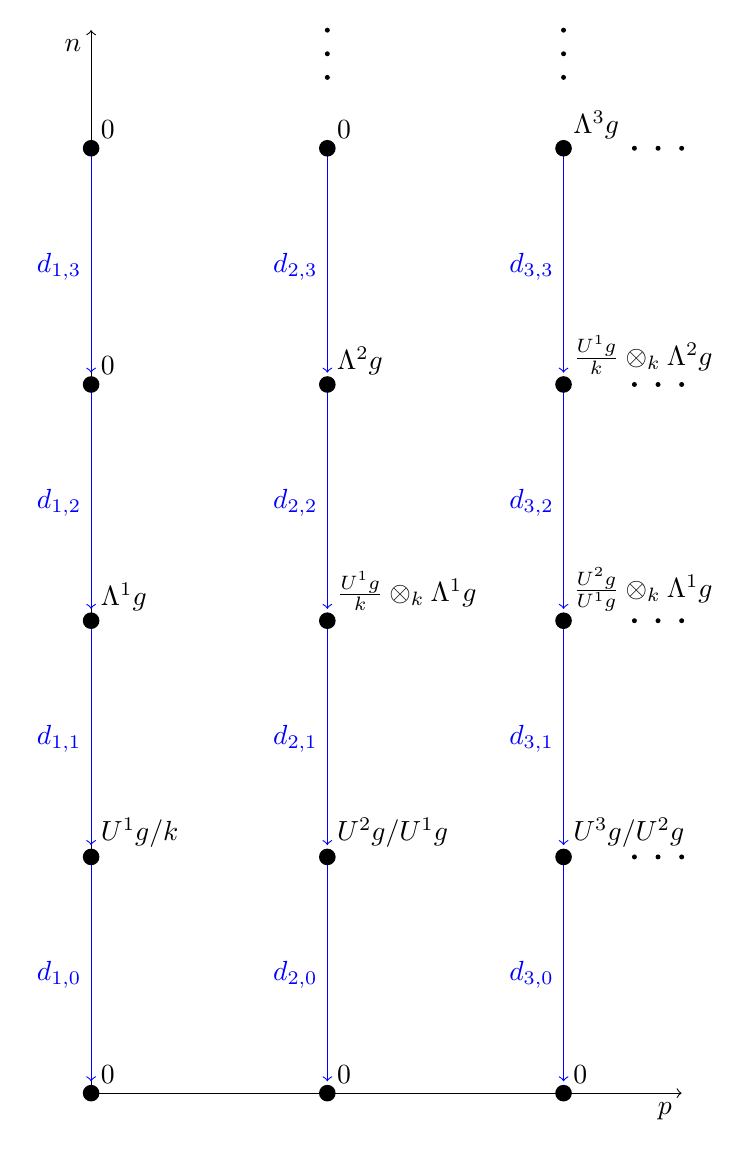
\begin{tikzpicture}[scale=3]  % Increased scale for better visibility
        % Grid dimensions
        \def\maxn{3} % Adjust as needed
        \def\minn{-1} % New minimum n value
        \def\maxp{3} % Adjust as needed
        \def\minp{1}  % Define minimum p value

        % Drawing the axes
        \draw[->] (\minp,-1) -- (\maxp+0.5,-1) node[anchor=north east] {$p$};
        \draw[->] (\minp,-1) -- (\minp,\maxn+0.5) node[anchor=north east] {$n$};

        % Drawing the lattice points, labels, and differential maps
        \foreach \n in {\minn,...,\maxn} {
          \foreach \p in {\minp,...,\maxp} {
            % Calculate p - 1 - n
            \pgfmathtruncatemacro{\diff}{\p - 1 - \n}
            \pgfmathtruncatemacro{\difff}{\p - \n}

            % Conditional structure for labeling
            \ifnum\n=-1
              \node[anchor=south west, black] at (\p,\n) {0}; % Special row for n = -1
            \else
              \ifnum\n>\p
                \node[anchor=south west, black] at (\p,\n) {0}; % Label as zero if n > p
              \else
                \ifnum\n=\p
                  \ifnum\n=0 % Special case for M_{0,0} = k
                    \node[anchor=south west, black] at (\p,\n) {$k$};
                  \else % Special case for diagonal (Lambda^n g)
                    \node[anchor=south west, black] at (\p,\n) {$\Lambda^\n \mathfrak{g}$};
                  \fi
                \else
                  \ifnum\n=0 % Special case for p-axis (p > 0, n = 0)
                    \ifnum\p=1
                      \node[anchor=south west, black] at (\p,\n) {$U^{\p}\mathfrak{g}/k$};
                    \else
                      \node[anchor=south west, black] at (\p,\n) {$U^{\p}\mathfrak{g}/U^{\diff}\mathfrak{g} $};
                    \fi
                  \else % General case
                    \ifnum\diff=0
                      \node[anchor=south west, black] at (\p,\n) {$\frac{U^{\difff}\mathfrak{g}}{k} \otimes_k \Lambda^\n \mathfrak{g}$};
                    \else
                      \node[anchor=south west, black] at (\p,\n) {$\frac{U^{\difff}\mathfrak{g}}{U^{\diff}\mathfrak{g}} \otimes_k \Lambda^\n \mathfrak{g}$};
                    \fi
                  \fi
                \fi
              \fi
            \fi

            % Draw differential maps (vertical arrows)
            \ifnum\n>-1
              \draw[->, blue] (\p,\n) -- (\p,\n-0.95); % Vertical differential
              \node[anchor=east, blue] at (\p,\n-0.5) {$d_{\p,\n}$};
            \fi

            % Draw lattice points
            \fill (\p,\n) circle (1pt);
          }
        }

        % Adding dots to indicate continuation
        \foreach \n in {0,...,\maxn} {
          \fill (\maxp+0.3,\n) circle (0.3pt);  % Dots on the right side
          \fill (\maxp+0.4,\n) circle (0.3pt);
          \fill (\maxp+0.5,\n) circle (0.3pt);
        }
        \foreach \p in {2,...,\maxp} {
          \fill (\p,\maxn+0.3) circle (0.3pt);  % Dots on the top side
          \fill (\p,\maxn+0.4) circle (0.3pt);
          \fill (\p,\maxn+0.5) circle (0.3pt);
        }
      \end{tikzpicture}
    \end{center}
    \caption{A small portion of $ W_{p, n} $ for $ 1 \leq p \leq 3 $ and $ -1 \leq n \leq 3 $ where the blue arrows are the induced differential maps on $ W_p $ which you get from the maps $ d_{p, n}:F_{p, n} \to F_{p, n-1} $. The chain complexes $ W_p $ are the direct sum of the components along the vertical direction.}\label{fig:filtration}
  \end{figure}


  Now, if we can show that $ W_p $ has trivial homology, then the long exact sequence induced from the short exact sequence in \ref{eq:ses} gives us that $ H_*(F_{p}) \cong H_{*}(F_{p-1}) $ for all $ p $. Since $ F_0 $ is just the trivial complex $ 0 \to k \to k \to 0 $ we have that $ H_*(F_0) = 0 $ and hence this would imply that $ H_*(F_p) = 0 $ for all $ p $ leading us to conclude that
  \begin{equation}
    H_*\left( V_*(\mathfrak{g})\xrightarrow{\epsilon} k \right) = \varinjlim{H_*(F_p)} = 0.
  \end{equation}

  What remains to show then is that $ H_*(W_p) = 0 $ for all $ p \geq 1 $. We do this explicitly by creating a chain homotopy $ s_{p, *}: W_{p, *} \to W_{p, *+1} $ between the identity and the zero map. Therefore, let $ I=(\alpha_1, \ldots, \alpha_{p - n} ) $ be an increasing sequence and $ J = (\beta_1, \ldots, \beta_n) $ a strictly increasing sequence. We then define $ s_{p, n} $ on basis elements $ \overline{e}_{I} \otimes e^{J} $ as follows:
  \begin{equation}
    s_{p, n}(\overline{e}_I \otimes e^{J}) = \begin{cases}
      (-1)^{n}\overline{e}_{(\alpha_1, \ldots, \alpha_{p - n - 1})}\otimes e^{(J, \alpha_{p - n})}, &\text{ if } \alpha_{p - n} > \beta_n\\
      0, &\text{ else.}
    \end{cases}
  \end{equation}
  Our goal is to show that
  \begin{equation}
    s_{p, n-1}d_{p, n} + d_{p, n+1}s_{p, n} = 1_{W_{p,n}}.
  \end{equation}
  Hence, let $ I = (\alpha_1, \ldots, \alpha_{p -n}) $ be an increasing sequence and $ J = (\beta_1, \ldots, \beta_n) $ a strictly increasing sequence. There are then two cases two consider, either $ \alpha_{p - n} > \beta_n $ or $ \alpha_{p - n} \leq \beta_n $. Assume first that $ \alpha_{p -n} > \beta_n $. We then have that
  \begin{align*}
    (s_{p, n-1}d_{p, n} + d_{p, n+1}s_{p, n})(\overline{e}_{I} \otimes e^{J}) &= s_{p, n-1}\left( \sum_{i = 1}^{n} (-1)^{i + 1}\overline{e}_{(I, \beta_i)} \otimes \wedge\left(e_{\beta_1}, \widehat{e}_{\beta_i}, e_{\beta_n}\right) \right) \\
                                                                            &\quad + d_{p, n-1}\left( (-1)^{n}\overline{e}_{(\alpha_1, \ldots, \alpha_{p-n-1})} \otimes e^{(J, \alpha_{p -n})} \right) \\
                                                                            &= \sum_{i = 1}^{n} (-1)^{i + n} \overline{e}_{(\alpha_1, \ldots, \alpha_{p - n - 1}, \beta_i)} \otimes \wedge\left(e_{\beta_1}, \widehat{e}_{\beta_i}, e_{\beta_n}, e_{\alpha_{p-n}} \right) \\
                                                                            &\quad + \sum_{i = 1}^{n} (-1)^{i + n + 1}\overline{e}_{(\alpha_1, \ldots, \alpha_{p-n-1}, \beta_i)} \otimes \wedge \left( e_{\beta_1}, \widehat{e}_{\beta_i}, e_{\beta_n}, e_{\alpha_{p - n}} \right) \\
                                                                            &\quad + \overline{e}_{I} \otimes e^{J} \\
                                                                            &= \overline{e}_{I} \otimes e^{J},
  \end{align*}
  where we use the fact that $ \alpha_{p - n} > \beta_i $ and so $ \overline{e}_{\alpha_1, \ldots, \alpha_{p - n}, \beta_i} = \overline{e}_{\alpha_1, \ldots, \beta_i, \alpha_{p - n}} $ in accordance with an earlier remark. The only important thing in the definition of $ s_{p, n} $ on basis elements is that the rightmost element in $ I $ is the largest one which is why we can apply $ s_{p, n-1} $ to $ \overline{e}_{(\alpha_1, \ldots, \alpha_{p -n - 1}, \beta_i, \alpha_{p -n})} \otimes \wedge \left( e_{\beta_1}, \widehat{e}_{\beta_i}, e_{\beta_n} \right) $ without much problem.

  On the other hand, assume that $ \alpha_{p - n} \leq \beta_n $. We then have that
  \begin{equation}
    s_{p, n}\left( e_{I} \otimes e^{J} \right) = 0
  \end{equation}
  and
  \begin{equation}
    s_{p, n -1} \left( \overline{e}_{(I, \beta_i)} \otimes \wedge \left( e_{\beta_1}, \widehat{e}_{\beta_i}, e_{\beta_n} \right) \right) = 0
  \end{equation}
  except for $ i = n $ where we have
  \begin{equation}
    s_{p, n -1}\left( e_{(I, \beta_n)} \otimes e^{(\beta_1, \ldots, \beta_{n - 1})} \right) = (-1)^{n - 1} \overline{e}_{I} \otimes e^{J}.
  \end{equation}
  From this it follows that
  \begin{align*}
    (s_{p, n-1}d_{p, n} + d_{p, n+1}s_{p, n})(\overline{e}_{I} \otimes e^{J}) &=  s_{p, n-1}\left( \sum_{i = 1}^{n} (-1)^{i + 1}\overline{e}_{(I, \beta_i)} \otimes \wedge\left(e_{\beta_1}, \widehat{e}_{\beta_i}, e_{\beta_n}\right) \right) + d_{p, n-1}(0) \\
                                                                              &= \sum_{i = 1}^{n} (-1)^{i + 1}s_{p, n-1}\left(\overline{e}_{(I, \beta_i)} \otimes \wedge\left(e_{\beta_1}, \widehat{e}_{\beta_i}, e_{\beta_n}\right)\right) \\
                                                                              &= (-1)^{n + 1 + n -1} \overline{e}_{I} \otimes e^{J} \\
                                                                              &= \overline{e}_{I} \otimes e^{J}
  \end{align*}
  as desired. We therefore see that $ s_{p, *}: W_{p, *} \to W_{p, *+1} $ is a chain homotopy between the identity and zero map on $ W_p $ which means that $ H_*(W_p) = 0 $. By earlier remarks this then implies that
  \begin{equation}
    H_*\left( V_*(\mathfrak{g})\xrightarrow{\epsilon} k \right) = 0
  \end{equation}
  showing that $ V_*(\mathfrak{g})\xrightarrow{\epsilon} k $ indeed is a projective resolution of $ k $ considered as a trivial $ \mathfrak{g} $-module (equivalently trivial $ U\mathfrak{g} $-module).
\end{proof}

\begin{corollary}[\cite{weibel1994homological}]
  \label{cor:cohom}
  If $ M $ is a right $ \mathfrak{g} $-module, then the homology modules $ H_*(\mathfrak{g}, M) $ are the homology of the chain complex
  \begin{equation}
    M \otimes_{U\mathfrak{g}} V_{*}(\mathfrak{g}) = M \otimes_{U\mathfrak{g}} U\mathfrak{g} \otimes_k \Lambda^{*}\mathfrak{g} = M \otimes_k \Lambda^{*}\mathfrak{g}.
  \end{equation}
  Similarly, if $ M $ is a left $ \mathfrak{g} $-module, then the cohomology modules $ H^{*}(\mathfrak{g}, M) $ are the cohomology of the cochain complex
  \begin{equation}
    \text{Hom}_{\mathfrak{g}\text{-}\mathbf{Mod}}(V_*(\mathfrak{g}), M) = \text{Hom}_{\mathfrak{g}\text{-}\mathbf{Mod}}(U\mathfrak{g} \otimes_k \Lambda^{*}\mathfrak{g}, M) \cong \text{Hom}_{k\text{-}\mathbf{Mod}}(\Lambda^{*}\mathfrak{g}, M).
  \end{equation}
  In this complex, an $ n $-cochain $ f: \Lambda^{n}\mathfrak{g} \to M $ is just an alternating $ k $-multilinear of $ n $ variables in $ \mathfrak{g} $, taking values in $ M $. The coboundary $ \delta f $ of such an $ n $-cochain is the $ (n +1) $-cochain given by
  \begin{align*}
    \delta f(e_{\alpha_1}, \ldots, e_{\alpha_n}, e_{\alpha_{n + 1}}) = &\sum_{i = 1}^{n} (-1)^{i + 1} e_{\alpha_i}f(e_{\alpha_1}, \ldots, \widehat{e}_{\alpha_i}, \ldots, e_{\alpha_n}, e_{\alpha_{n + 1}}) \\
                                                                       &+ \sum_{i < j} (-1)^{i + j} f \left( [e_{\alpha_i}, e_{\alpha_{j}}], e_{\alpha_1}, \ldots, \widehat{e}_{\alpha_i}, \ldots, \widehat{e}_{\alpha_j}, \ldots, e_{\alpha_n}, e_{\alpha_{n + 1}} \right).
  \end{align*}
\end{corollary}
% subsection The Chevalley-Eilenberg Complex (end)

\subsection{$ H^2 $ and extensions} % (fold)
\label{sub:H^2 and extensions}
Corollary~\ref{cor:cohom} gives us a concrete and practical way of calculating the Lie algebra (co)homology for a wide array of Lie algebras $ \mathfrak{g} $ and $ \mathfrak{g} $-modules $ M $. However, in the special case of wanting to compute $ H^2(\mathfrak{g}, M) $ we can classify the cohomology in another way, namely as equivalence classes of Lie algebra extensions of $ \mathfrak{g} $ by $ M $. For this to make sense we need to understand what we mean by such an extension.
\begin{definition}[Extension of a Lie algebra]
  Let $ \mathfrak{g} $ and $ \mathfrak{h} $ be two Lie algebras. An \textbf{extension} of $ \mathfrak{g} $ by $ \mathfrak{h} $ is a short exact sequence of Lie algebras:
  \begin{equation}
    \label{eq:lieextension}
    0 \to \mathfrak{h} \xrightarrow{i} \mathfrak{e} \xrightarrow{p} \mathfrak{g} \to 0.
  \end{equation}
  Two such extensions of $ \mathfrak{g} $ by $ \mathfrak{h} $ are said to be equivalent if there exist a Lie algebra homomorphism $ \varphi: \mathfrak{e} \to \mathfrak{e}' $ which makes the following diagram commute:
  \[\begin{tikzcd}
	  0 & {\mathfrak{h}} & {\mathfrak{e}} & {\mathfrak{g}} & 0 \\
	  0 & {\mathfrak{h}} & {\mathfrak{e}'} & {\mathfrak{g}} & 0.
	  \arrow[Rightarrow, no head, from=1-4, to=2-4]
	  \arrow["\varphi", from=1-3, to=2-3]
	  \arrow[from=1-1, to=1-2]
	  \arrow["i", from=1-2, to=1-3]
	  \arrow["p", from=1-3, to=1-4]
	  \arrow[from=1-4, to=1-5]
	  \arrow["{i'}"', from=2-2, to=2-3]
	  \arrow["{p'}"', from=2-3, to=2-4]
	  \arrow[from=2-1, to=2-2]
	  \arrow[from=2-4, to=2-5]
	  \arrow[Rightarrow, no head, from=1-2, to=2-2]
  \end{tikzcd}\]
  The five-lemma implies that $ \varphi $ must necessarily be an isomorphism.
\end{definition}

\begin{definition}[Split extension]
  An extension of the form in \ref{eq:lieextension} is called \textbf{split} if there exists a Lie algebra homomorphism $ \tau: \mathfrak{g} \to \mathfrak{e} $ such that $ p \circ \tau = 1_\mathfrak{g} $.
\end{definition}

Before we properly define what we mean by an extension of $ \mathfrak{g} $ by a $ \mathfrak{g} $-module $ M $ we need to talk about semidirect products.
\begin{definition}[Semidirect product]
  Let $ \mathfrak{g} $ be a Lie algebra and $ M $ a $ \mathfrak{g} $-module. The semidirect product of $ M $ and $ \mathfrak{g} $, denoted $ M \rtimes \mathfrak{g} $, is the Lie algebra with underlying $ k $-module structure $ M \oplus \mathfrak{g} $ and Lie bracket given by
  \begin{equation}
    [(m, x), (n, y)] = \left(xn - ym, [x, y]\right).
  \end{equation}
\end{definition}
Now, let $ M $ be an abelian Lie algebra and $ \mathfrak{e} $ and extension of $ \mathfrak{g} $ by $ M $. This means we have a short exact sequence of the form
\begin{equation}
  0 \to M \xrightarrow{i} \mathfrak{e} \xrightarrow{p} \mathfrak{g} \to 0.
\end{equation}
We can then give $ M $ a $ \mathfrak{g} $-module structure as follows. For $ x \in \mathfrak{g} $ and $ m \in M $ let
\begin{equation}
  xm = i^{-1}\left( [\pi^{-1}(x), i(m)] \right).
\end{equation}
To see why this is well defined, suppose $ \pi(e) = x = \pi(e') $. Then $ \pi(e - e') = 0 $ and by exactness there then exists an $ m' \in M $ such that $ i(m')=e - e' $. However, this implies that
\begin{align*}
  i^{-1}\left( [e, i(m)] \right) - i^{-1}(\left( [e', i(m)] \right)) &= i^{-1}\left( [e - e', i(m)] \right) \\
                                                                     &= i^{-1}(i([m', m])) \\
                                                                     &= i^{-1}(i(0)) \\
                                                                     &= 0
\end{align*}
showing that $ xm $ is well defined. The interesting case is when $ M $ already has a $ \mathfrak{g} $-module. In this case we can form the extension of $ \mathfrak{g} $ by $ M $ by taking the semidirect product of $ M $ and $ \mathfrak{g} $ and give $ M $ a new $ \mathfrak{g} $-module structure from $ M \rtimes \mathfrak{g} $.
\begin{lemma}
  Let $ M $ be a $ \mathfrak{g} $-module. Then the induced $ \mathfrak{g} $-module structure on $ M $ which we get from the short exact sequence
  \begin{equation}
    0 \to M \xrightarrow{\iota} M \rtimes \mathfrak{g} \xrightarrow{\pi} \mathfrak{g} \to 0
  \end{equation}
  coincides with the original $ \mathfrak{g} $-module structure.
\end{lemma}
\begin{proof}
  We choose $ (0, x) $ as the representative for $ \pi^{-1}(x) $. We then have that
  \begin{align*}
    \iota^{-1}\left( [\pi^{-1}(x), i(m)] \right) &= \iota^{-1}\left( [(0,x), (m, 0)] \right) \\
                                             &= \iota^{-1}\left(xm - 0\cdot0, [0,0]\right) \\
                                             &= \iota^{-1}((xm, 0)) \\
                                             &= xm
  \end{align*}
  showing that they coincide.
\end{proof}
We can now state the theorem we want to show.

\begin{theorem}
  \label{thm:equivalence}
  Let $ \mathfrak{g} $ be a Lie algebra over $ k $ and $ M $ a $ \mathfrak{g} $-module. Then the elements of $ H^2(\mathfrak{g}, M) $ are in a natural one-to-one correspondence with the set of equivalence classes of Lie algebra extensions of $ \mathfrak{g} $ by $ M $ that induce the same fixed $ \mathfrak{g} $-module structure.
\end{theorem}
We delay the proof of this theorem to follow the path suggested in \cite[Exercise 7.7.5]{weibel1994homological} and prove some lemmas first.

\begin{lemma}
  Let $ M $ be a $ \mathfrak{g} $-module. If $ 0 \to M \xrightarrow{i} \mathfrak{e} \xrightarrow{p} \mathfrak{g} \to 0 $ is an extension of Lie algebras that induce the same $ \mathfrak{g} $-module structure on $ M $, and $ \sigma: \mathfrak{g} \to \mathfrak{e} $ is a $ k $-module splitting of $ p $ (such a splitting exists as $ \mathfrak{g} $ is free) then the Lie algebra structure on $ \mathfrak{e} \cong M \oplus \mathfrak{g} $ may be described by an alternating $ k $-bilinear function $ \omega: \mathfrak{g} \times \mathfrak{g} \to M $ defined by
  \begin{equation}
    \omega(x,y) = i^{-1}\left([\sigma(x), \sigma(y)] - \sigma \left( [x, y] \right)\right), \quad\quad \forall x,y \in \mathfrak{g}.
  \end{equation}
  Moreover, $ \omega $ is a cochain, meaning that $ \delta \omega = 0 $.
\end{lemma}
\begin{proof}
  First of all, notice that the definition of $ \omega $ makes sense as applying $ p $ to the inner argument of $ i^{-1} $ gives $ 0 $ and hence there must exist an element $ m \in M $ such that $ i(m)=i(\omega(x,y)) $.

  Next, some conventions: let $ xm $ denote the original $ \mathfrak{g} $-module action of $ \mathfrak{g} $ on $ M $ and let $ x_{\mathfrak{e}} m $ denote the $ \mathfrak{g} $-module action of $ \mathfrak{g} $ on $ M $ induced by the Lie algebra extension. By assumption we then have $ x_{\mathfrak{e}}m = xm $ for all $ x \in \mathfrak{g} $ and $ m \in M $. Next, let
  \begin{equation}
    0 \to M \xrightarrow{\iota} M \rtimes \mathfrak{g} \xrightarrow{\pi} \mathfrak{g} \to 0
  \end{equation}
  be the short exact sequence of Lie algebras you get from taking the semidirect product of $ M $ and $ \mathfrak{g} $.

  The $ k $-module isomorphism $ \psi: M \oplus \mathfrak{g} \to \mathfrak{g} $ is then given on elements by
  \begin{equation}
    \psi(m , x) = i(m) + \sigma(x),\quad \forall (m,x) \in M \oplus \mathfrak{g}
  \end{equation}
  and
  \begin{equation}
    \psi^{-1}(d) = (i^{-1}(d - \sigma(p(d))), p(d)), \quad \forall d \in \mathfrak{e}.
  \end{equation}
  This implies that the Lie algebra structure on $ M \oplus \mathfrak{g} $ is given by
  \begin{equation}
    [(m, x), (n, y)] = \psi^{-1}\left( [\psi(m, x), \psi(n, y)] \right),
    \quad \forall (m,x),(n,y) \in M \oplus \mathfrak{g}
  .\end{equation}
  Expanding this out we have
  \begin{align*}
    [(m, x), (n, y)] &= \psi^{-1}\left( [i(m) + \sigma(x),  i(n) + \sigma(y)] \right) \\
                     &= \psi^{-1}\left( i([m, n]) + [\sigma(x), i(n)] - [\sigma(y), i(m)] + [\sigma(x), \sigma(y)] \right) \\
                     &=\psi^{-1}\left( i(x_{\mathfrak{e}} n - y_{\mathfrak{e}} m ) + [\sigma(x), \sigma(y)] \right) \\
                     &= (x_{\mathfrak{e}}n - y_{\mathfrak{e}}m + i^{-1}(\left( [\sigma(x), \sigma(y)] \right) - \sigma([x, y])), [x, y])\\
                     &= (x_{\mathfrak{e}}n - y_{\mathfrak{e}}m +\omega(x,y), [x, y])
  \end{align*}
  showing that the Lie algebra structure on $ M \oplus \mathfrak{g} \cong \mathfrak{e} $ indeed is given by the $ k $-bilinear alternating function
  \begin{equation}
    \omega(x,y) = i^{-1}([\sigma(x), \sigma(y)] - \sigma([x,y])).
  \end{equation}

  Next to see that $ \delta \omega = 0 $, let $ x,y,z \in \mathfrak{g} $. In the following we shall use $ \sigma(x), \sigma(y), \sigma(z) $ as canditates for $ p^{-1}(x)$, $p ^{-1}(y), $ and $ p ^{-1}(z) $ respectively. Corollary~\ref{cor:cohom} now implies that
  \begin{align*}
    \delta \omega (x,y,z) &= x\omega(y, z) - y\omega(x, z) + z\omega(x,y) \\
                          &\quad -\omega([x,y], z) + \omega([x,z], y) - \omega([y,z], x) \\ \\
                          &= x i^{-1}([\sigma(y), \sigma(z)] - \sigma([y,z])) \\
                          &\quad -yi^{-1}([\sigma(x), \sigma(z)] - \sigma([x,z])) \\
                          &\quad +zi^{-1}([\sigma(x), \sigma(y)]- \sigma([x,y])) \\
                          &\quad - i^{-1}([\sigma([x, y]), \sigma(z)]-\sigma([[x,y], z])) \\
                          &\quad + i^{-1}([\sigma([x, z]), \sigma(y)] -\sigma([[x,z], y])) \\
                          &\quad - i^{-1}([\sigma([y, z]), \sigma(x)] -\sigma([[y,z], x])) \\ \\
                          &= x_{\mathfrak{e}}i^{-1}([\sigma(y), \sigma(z)] - \sigma([y,z])) \\
                          &\quad -y_{\mathfrak{e}}i^{-1}([\sigma(x), \sigma(z)] - \sigma([x,z])) \\
                          &\quad +z_{\mathfrak{e}}i^{-1}([\sigma(x), \sigma(y)]- \sigma([x,y])) \\
                          &\quad - i^{-1}([\sigma([x, y]), \sigma(z)]-\sigma([[x,y], z])) \\
                          &\quad + i^{-1}([\sigma([x, z]), \sigma(y)] -\sigma([[x,z], y])) \\
                          &\quad - i^{-1}([\sigma([y, z]), \sigma(x)] -\sigma([[y,z], x])) \\ \\
                          &= i^{-1}([\sigma(x), [\sigma(y), \sigma(z)]] - [\sigma(x), \sigma([y, z])]) \\
                          &\quad - i^{-1}([\sigma(y), [\sigma(x), \sigma(z)]] - [\sigma(y), \sigma([x, z])]) \\
                          &\quad + i^{-1}([\sigma(z), [\sigma(x), \sigma(y)]] - [\sigma(z), \sigma([x, y])]) \\
                          &\quad - i^{-1}([\sigma([x, y]), \sigma(z)]-\sigma([[x,y], z]) \\
                          &\quad + i^{-1}([\sigma([x, z]), \sigma(y)] -\sigma([[x,z], y])) \\
                          &\quad - i^{-1}([\sigma([y, z]), \sigma(x)] -\sigma([[y,z], x])) \\ \\
                          &= i^{-1}([\sigma(x), [\sigma(y), \sigma(z)]] - [\sigma(x), \sigma([y, z])] \\
                          &\quad\quad\quad - [\sigma(y), [\sigma(x), \sigma(z)]] + [\sigma(y), \sigma([x, z])] \\
                          &\quad\quad\quad + [\sigma(z), [\sigma(x), \sigma(y)]] - [\sigma(z), \sigma([x, y])] \\
                          &\quad\quad\quad - [\sigma([x, y]), \sigma(z)]+\sigma([[x,y], z]) \\
                          &\quad\quad\quad + [\sigma([x, z]), \sigma(y)] -\sigma([[x,z], y]) \\
                          &\quad\quad\quad - [\sigma([y, z]), \sigma(x)] +\sigma([[y,z], x]))
  \end{align*}
  The Jacobi identity implies that both
  \begin{align*}
    \sigma([[x,y], z]) - \sigma([[x, z], y]) + \sigma([[y,z], x]) &= \sigma([[x,y], z]) + \sigma([[z, x], y]) + \sigma([[y,z], x]) \\&= 0
  \end{align*}
  and
  \begin{align*}
    &[\sigma(x), [\sigma(y), \sigma(z)]] -
    [\sigma(y), [\sigma(x), \sigma(z)]] +
    [\sigma(z), [\sigma(x), \sigma(y)]]\\ &=
    [\sigma(x), [\sigma(y), \sigma(z)]] +
    [\sigma(y), [\sigma(z), \sigma(x)]] +
    [\sigma(z), [\sigma(x), \sigma(y)]]\\ &= 0
  \end{align*}
  so that the terms on the diagonal in the expression for $ \delta\omega(x,y,z) $. Hence we have
  \begin{align*}
    \delta\omega(x,y,z) &= i^{-1}([\sigma(x), [\sigma(y), \sigma(z)]] - [\sigma(x), \sigma([y, z])] \\
                          &\quad\quad\quad - [\sigma(y), [\sigma(x), \sigma(z)]] + [\sigma(y), \sigma([x, z])] \\
                          &\quad\quad\quad + [\sigma(z), [\sigma(x), \sigma(y)]] - [\sigma(z), \sigma([x, y])] \\
                          &\quad\quad\quad - [\sigma([x, y]), \sigma(z)]+\sigma([[x,y], z]) \\
                          &\quad\quad\quad + [\sigma([x, z]), \sigma(y)] -\sigma([[x,z], y]) \\
                          &\quad\quad\quad - [\sigma([y, z]), \sigma(x)] +\sigma([[y,z], x])) \\
                          &= i^{-1}(- [\sigma(x), \sigma([y, z])] \\
                          &\quad\quad\quad + [\sigma(y), \sigma([x, z])] \\
                          &\quad\quad\quad - [\sigma(z), \sigma([x, y])] \\
                          &\quad\quad\quad - [\sigma([x, y]), \sigma(z)] \\
                          &\quad\quad\quad + [\sigma([x, z]), \sigma(y)] \\
                          &\quad\quad\quad - [\sigma([y, z]), \sigma(x)]) \\
                          &= i^{-1}(0) \\
                          &= 0
  \end{align*}
  showing that $ \delta\omega $ is a cochain as desired.
\end{proof}

Next we show that the $ \omega $ constructed above gives a well defined class $ [\omega] \in H^{2}(\mathfrak{g}, M) $ for a given Lie algebra extension.
\begin{lemma}
  If $ \sigma' $ is any other $ k $-module splitting of $ p $ in $ 0 \to M \xrightarrow{i} \mathfrak{e} \xrightarrow{p} \mathfrak{g} \to 0 $ then the resulting 2-cocycle $ \omega' $ is cohomologous to $ \omega $.
\end{lemma}
\begin{proof}
  Let $ \tau = \sigma - \sigma' $. As $ \text{Hom}_{k\text{-}\mathbf{Mod}}(\mathfrak{g}, -) $ is left exact we have another exact sequence
  \begin{equation}
    0 \to  \text{Hom}_{k\text{-}\mathbf{Mod}}(\mathfrak{g}, M) \xrightarrow{i_{*}}  \text{Hom}_{k\text{-}\mathbf{Mod}}(\mathfrak{g}, \mathfrak{e}) \xrightarrow{p_*}  \text{Hom}_{k\text{-}\mathbf{Mod}}(\mathfrak{g}, \mathfrak{g}).
  \end{equation}
  Then, as
  \begin{align*}
    p_*(\tau) &= p(\sigma - \sigma') \\
              &= p \sigma - p \sigma' \\
              &= 1_\mathfrak{g} - 1_\mathfrak{g} \\
              &= 0
  \end{align*}
  there must exist, by exactness, an $ \epsilon \in  \text{Hom}_{k\text{-}\mathbf{Mod}}(\mathfrak{g}, M)  $ such that $ i \circ \epsilon = \tau $. We claim that $ \omega - \omega' = \delta\epsilon $. To see this, let $ x,y \in \mathfrak{g} $, then
  \begin{align*}
    (\omega - \omega')(x,y) &= i^{-1}([\sigma(x), \sigma(y)] - \sigma([x,y])) \\
                            &\quad - i^{-1}([\sigma'(x), \sigma'(y)] - \sigma'([x,y])) \\
                            &= i^{-1}([\sigma(x), \sigma(y)] - \sigma([x,y]) \\
                            &\quad\quad -[\sigma'(x), \sigma'(y)] + \sigma'([x,y])) \\
                            &= i^{-1}([\sigma(x), \sigma(y)] - [\sigma'(x), \sigma(y)] \\
                            &\quad\quad +[\sigma'(x), \sigma(y)] - [\sigma'(x), \sigma'(y)] \\
                            &\quad\quad - \tau([x,y])) \\
                            &= i^{-1}([\sigma'(x), \tau(y)] - [\sigma(y), \tau(x)]- \tau([x,y])) \\
                            &= i^{-1}(i(x_\mathfrak{e}\epsilon(y)) - i(y_{\mathfrak{e}}\epsilon(x)) - i(\epsilon([x,y]))) \\
                            &= i^{-1}(i(x\epsilon(y) - y\epsilon(x) - \epsilon([x,y]))) \\
                            &= x\epsilon(y) - y\epsilon(x) - \epsilon([x,y]) \\
                            &= \delta\epsilon(x,y)
  \end{align*}
  showing that $ \omega $ and $ \omega' $ are cohomologous.
\end{proof}
The above lemma shows that every Lie algebra extensions defines a unique element in $ H^2(\mathfrak{g}, M) $. Next we want to show that equivalent extensions give the same element.

\begin{lemma}
  Let $ \psi: \mathfrak{e}_\omega \to \mathfrak{e}_{\omega'} $ be an equivalence of Lie algebra extensions of $ \mathfrak{g} $ by $ M $, i.e., there is a commutative diagram
  \[\begin{tikzcd}
	  0 & M & {\mathfrak{e}_\omega} & {\mathfrak{g}} & 0 \\
	  0 & M & {\mathfrak{e}_{\omega'}} & {\mathfrak{g}} & 0.
	  \arrow[Rightarrow, no head, from=1-4, to=2-4]
	  \arrow["\psi", from=1-3, to=2-3]
	  \arrow[from=1-1, to=1-2]
	  \arrow["i", from=1-2, to=1-3]
	  \arrow["p", from=1-3, to=1-4]
	  \arrow[from=1-4, to=1-5]
	  \arrow["{i'}"', from=2-2, to=2-3]
	  \arrow["{p'}"', from=2-3, to=2-4]
	  \arrow[from=2-1, to=2-2]
	  \arrow[from=2-4, to=2-5]
	  \arrow[Rightarrow, no head, from=1-2, to=2-2]
  \end{tikzcd}\]
  Then the two corresponding classes of the extensions, i.e., $ \omega $ and $ \omega' $, are cohomologous.
\end{lemma}
\begin{proof}
  As both $ \mathfrak{e}_{\omega} $ and $ \mathfrak{e}_{\omega'} $ splits as $ k $-modules, we have the following commutative diagram of $ k $-modules:
  \[\begin{tikzcd}
	  0 & M & {M\oplus\mathfrak{g}} & {\mathfrak{g}} & 0 \\
	  0 & M & {\mathfrak{e}_\omega} & {\mathfrak{g}} & 0 \\
	  0 & M & {\mathfrak{e}_{\omega'}} & {\mathfrak{g}} & 0 \\
	  0 & M & {M\oplus\mathfrak{g}} & {\mathfrak{g}} & 0
	  \arrow[from=1-1, to=1-2]
	  \arrow["\iota", from=1-2, to=1-3]
	  \arrow["\pi", from=1-3, to=1-4]
	  \arrow[from=1-4, to=1-5]
	  \arrow[from=2-1, to=2-2]
	  \arrow[from=3-1, to=3-2]
	  \arrow[from=4-1, to=4-2]
	  \arrow["i", from=2-2, to=2-3]
	  \arrow["p", from=2-3, to=2-4]
	  \arrow[from=2-4, to=2-5]
	  \arrow["\iota", from=4-2, to=4-3]
	  \arrow["{i'}", from=3-2, to=3-3]
	  \arrow["{p'}", from=3-3, to=3-4]
	  \arrow["\pi", from=4-3, to=4-4]
	  \arrow[from=4-4, to=4-5]
	  \arrow[from=3-4, to=3-5]
	  \arrow[Rightarrow, no head, from=1-4, to=2-4]
	  \arrow[Rightarrow, no head, from=2-4, to=3-4]
	  \arrow[Rightarrow, no head, from=3-4, to=4-4]
	  \arrow["{\varphi_\omega}", from=1-3, to=2-3]
	  \arrow["\psi", from=2-3, to=3-3]
	  \arrow["{\varphi_{\omega'}^{-1}}", from=3-3, to=4-3]
	  \arrow[Rightarrow, no head, from=1-2, to=2-2]
	  \arrow[Rightarrow, no head, from=2-2, to=3-2]
	  \arrow[Rightarrow, no head, from=3-2, to=4-2]
  \end{tikzcd}\]
  where $ \varphi_\omega $ and $ \varphi_{\omega'} $ are the induced $ k $-module isomorphism from the splittings $ \sigma:\mathfrak{g} \to \mathfrak{e}_{\omega} $ and $ \sigma':\mathfrak{g} \to \mathfrak{e}_{\omega'} $ respectively. Consider the composition $ \varphi_{\omega'}^{-1} \circ \psi \circ \varphi_{\omega} \in \text{End}_{k\text{-}\mathbf{Mod}}(M \oplus \mathfrak{g}) $. On elements $ (m,x) \in M \oplus \mathfrak{g} $ it is given by
  \begin{align*}
    (\varphi_{\omega'}^{-1} \circ \psi \circ \varphi_{\omega})(m,x) &= (\varphi_{\omega'}^{-1} \circ \psi)(i(m) + \sigma(x)) \\
                                                                    &= \varphi_{\omega'}^{-1}(i'(m) + \psi(\sigma(x))) \\
                                                                    &= (i'^{-1}(i'(m) + \psi(\sigma(x)) -\sigma'(x)), x) \\
                                                                    &= (m + i'^{-1}(\psi(\sigma(x)) - \sigma'(x)),x)
  \end{align*}
  where the last equality is allowed as $ p'(\psi(\sigma(x)))-p'(\sigma'(x)) =0$. However, by exactness of the corresponding hom-sequence, this must mean that there is some $ k $-module homomorphism $ \epsilon: \mathfrak{g} \to M$ such that $ i'\circ \epsilon = \psi\circ \sigma - \sigma' $ and we can therefore write
  \begin{equation}
    (\varphi_{\omega'}^{-1} \circ \psi \circ \varphi_{\omega})(m,x) = (m + \epsilon(x), x).
  \end{equation}
  Letting the $ M \oplus \mathfrak{g} $ have the Lie algebra structure induced by $ \mathfrak{e}_{\omega} $ and the $ M \oplus \mathfrak{g} $ at the bottom have the Lie algebra structure induced by $ \mathfrak{e}_{\omega'} $ we get that both $ \varphi_\omega $ and $ \varphi_{\omega'} $ turn into Lie algebra isomorphism and consequently the above diagram is a commutative diagram of Lie algebras.

  Let $ \Psi = \varphi_{\omega'}^{-1} \circ \psi \circ \varphi_\omega $ and note that it is a Lie algebra isomorphism. This in turn means that, given $ (m,x),(n,y) \in M\oplus \mathfrak{g} $, we have
  \begin{equation}
    \Psi([(m, x), (n,y)]) = [\Psi(m, x), \Psi(n, y)].
  \end{equation}
  Now, we have that
  \begin{align*}
    \Psi([(m, x), (n, y)]) &= \Psi(x_{\mathfrak{e}_\omega}n - y_{\mathfrak{e}_\omega}m + \omega(x,y), [x,y]) \\
                           &= (xn - ym + \omega(x,y) + \epsilon([x,y]), [x,y])
  \end{align*}
  where we used the fact that $ x_{\mathfrak{e}_\omega}n = xn $, and we also have
  \begin{align*}
    [\Psi(m, x), \Psi(n, y)] &= [(m + \epsilon(x),x) (n + \epsilon(y), y)] \\
                             &= (x_{\mathfrak{e}_{\omega'}}n + x_{\mathfrak{e}_{\omega'}}\epsilon(y) - y_{\mathfrak{e}_{\omega'}}m - y_{\mathfrak{e}_{\omega'}}\epsilon(x) + w'(x,y), [x,y])\\
                             &= (xn -ym +x\epsilon(y) - y\epsilon(x) + \omega'(x,y), [x,y]).
  \end{align*}
  Equating these two we must have
  \begin{align*}
    xn - ym + \omega(x,y) + \epsilon([x,y] &= xn -ym +x\epsilon(y) - y\epsilon(x) + \omega'(x,y)\\
                                                     &\Updownarrow \\
    (\omega - \omega')(x,y)&= x\epsilon(y) - y\epsilon(x) - \epsilon([x,y]) \\
                           &= \delta \epsilon(x,y)
  \end{align*}
  showing that $ \omega $ and $ \omega' $ are cohomologous. Thus, equivalent extensions give cohomologous $ 2 $-cocycles and hence induce the same class in $ H^2(\mathfrak{g}, M) $.
\end{proof}

\begin{proof}[Proof of Theorem~\ref{thm:equivalence}]
  We have seen that there is a well defined map $ \Xi: \text{Ext}_{\text{Lie}}(\mathfrak{g}, M) \to H^2(\mathfrak{g}, M) $, where $ \text{Ext}_{\text{Lie}}(\mathfrak{g}, M) $ is the set of equivalence classes of Lie algebra extensions of $ \mathfrak{g} $ by M. Thus, what we must now do is create an inverse map $ \zeta: H^2(\mathfrak{g}, M) \to \text{Ext}_{\text{Lie}}(\mathfrak{g}, M) $.

  To this end, let $ [\omega] \in H^2(\mathfrak{g}, M) $ and define the Lie algebra $ \mathfrak{g}_\omega $ as follows: the underlying $ k $-module structure of $ \mathfrak{g}_\omega $ is $ M \oplus \mathfrak{g} $ and the Lie algebra bracket is given by
  \begin{equation}
    [(m, x), (n, y)] = (xn - ym + \omega(x,y), [x,y]).
  \end{equation}
  To see that it satisfies the Jacobi identity, let $ m_1, m_2, m_3 \in M $ and $ x_1, x_2, x_3 \in \mathfrak{g} $. Note that we only need to worry about the first component as the Jacobi identity for $ [-, -] $ on $ \mathfrak{g} $ takes care of the second component. In any case, we have that the first component of the summands in
  \begin{align*}
    &[(m_1, x_1), [(m_2, x_2), (m_3, x_3)]]\\+ &
    [(m_2, x_2), [(m_3, x_3), (m_1, x_1)]]\\ +&
    [(m_3, x_3), [(m_1, x_1), (m_2, x_2)]]
  \end{align*}
  are given by
  \begin{align*}
    [(m_1, x_1), [(m_2, x_2), (m_3, x_3)]]_1 &= x_1x_2m_3 - x_1x_3m_2 + x_1\omega(x_2, x_3) - [x_2, x_3]m_1 + \omega([x_1, [x_2, x_3]])\\
    [(m_2, x_2), [(m_3, x_3), (m_1, x_1)]]_1 &= x_2x_3m_1 - x_3x_2m_1 + x_2\omega(x_3, x_1) - [x_3, x_1]m_2 +\omega([x_2, [x_3, x_1]])\\
    [(m_3, x_3), [(m_1, x_1), (m_2, x_2)]]_1 &= x_3x_1m_2 - x_2x_1m_3 + x_3\omega(x_1, x_2) - [x_1, x_2]m_3 + \omega([x_3, [x_1, x_2]])
  \end{align*}
  which taken together becomes
  \begin{align*}
    &\quad x_1x_2m_3 - x_1x_3m_2 + x_1\omega(x_2, x_3) - [x_2, x_3]m_1 + \omega(x_1, [x_2, x_3])\\
    &\quad+x_2x_3m_1 - x_3x_2m_1 + x_2\omega(x_3, x_1) - [x_3, x_1]m_2 + \omega([x_2, [x_3, x_1]]) \\
    &\quad+x_3x_1m_2 - x_2x_1m_3 + x_3\omega(x_1, x_2) - [x_1, x_2]m_3 + \omega([x_3, [x_1, x_2]]) \\
    &= [x_1, x_2]m_3 - [x_1, x_2]m_3 \\
    &\quad +[x_2, x_3]m_1 - [x_2, x_3]m_1 \\
    &\quad +[x_3, x_1]m_2 - [x_3, x_1]m_2 \\
    &\quad + x_1\omega(x_2, x_3) - x_2 \omega(x_1, x_3) +x_3\omega(x_1, x_2) \\
    &\quad -\omega([x_2, x_3], x_1) + \omega([x_1, x_3], x_2) - \omega([x_1, x_2], x_3) \\
    &= x_1\omega(x_2, x_3) - x_2 \omega(x_1, x_3) +x_3\omega(x_1, x_2)
     -\omega([x_2, x_3], x_1) + \omega([x_1, x_3], x_2) - \omega([x_1, x_2], x_3) \\
    &=\delta\omega(x_1, x_2, x_3)\\
    &= 0
  \end{align*}
  showing that the bracket does indeed satisfy the Jacobi identity. We let the extension be the canonical short exact sequence
  \begin{equation}
    0 \to M \xrightarrow{\iota} \mathfrak{g}_{\omega} \xrightarrow{\pi} \mathfrak{g} \to 0
  \end{equation}
  where $ \iota $ is the inclusion $ m \mapsto (m, 0) $ and $ \pi $ is the projection $ (m, x) \mapsto x $.

  We must now show that cohomologous 2-cocycles $ \omega $ and $ \omega' $ give rise to equivalent Lie algebra extensions $ \mathfrak{g}_\omega $ and $ \mathfrak{g}_{\omega'} $. Thus, suppose $ \omega - \omega' = \delta\epsilon $ for some $ \epsilon \in \text{Hom}_{k\text{-}\mathbf{Mod}}(\mathfrak{g}, M) $. Define the $ k $-module map $ \psi: \mathfrak{g}_{\omega} \to \mathfrak{g}_{\omega'} $ by $ \psi(m, x) = (m + \epsilon(x), x) $. This is clearly an isomorphism of $ k $-modules but we need to show that
  \begin{equation}
    \psi([(m, x), (n, y)]) = [\psi(m, x), \psi(n, y)].
  \end{equation}
  The left hand side above is given by
  \begin{align*}
    \psi([(m, x), (n, y)]) &= \psi(xn - ym + \omega(x, y), [x,y]) \\
                           &= (xn - ym + \omega(x, y) + \epsilon([x,y]), [x,y])
  \end{align*}
  while the right hand side is
  \begin{align*}
    [\psi(m, x), \psi(n, y)] &= [(m + \epsilon(x), x), (n + \epsilon(y), y)] \\
                             &= (xn - ym + x\epsilon(y)- y\epsilon(x) + \omega'(x,y), [x,y])
  .\end{align*}
  We thus see that their second components are equal, and taking the difference of the first components we have
  \begin{align*}
  &\quad xn - ym + \omega(x, y) + \epsilon([x,y]) \\
  &\quad-xn +ym - x\epsilon(y) +y\epsilon(x) - \omega'(x,y) \\
  &= (\omega - \omega')(x, y) - \delta\epsilon(x,y) \\
  &= 0
  \end{align*}
  showing that $ \psi $ is an isomorphism of Lie algebras. Moreover, $ \psi $ fits into the following commutative diagram
  \[\begin{tikzcd}
	  0 & M & {\mathfrak{g}_\omega} & {\mathfrak{g}} & 0 \\
	  0 & M & {\mathfrak{g}_{\omega'}} & {\mathfrak{g}} & 0.
	  \arrow[Rightarrow, no head, from=1-4, to=2-4]
	  \arrow["\psi", from=1-3, to=2-3]
	  \arrow[from=1-1, to=1-2]
	  \arrow["\iota", from=1-2, to=1-3]
	  \arrow["\pi", from=1-3, to=1-4]
	  \arrow[from=1-4, to=1-5]
	  \arrow["{\iota}"', from=2-2, to=2-3]
	  \arrow["{\pi}"', from=2-3, to=2-4]
	  \arrow[from=2-1, to=2-2]
	  \arrow[from=2-4, to=2-5]
	  \arrow[Rightarrow, no head, from=1-2, to=2-2]
  \end{tikzcd}\]
  showing that we have a well defined map $ \zeta: H^2(\mathfrak{g}, M) \to \text{Ext}_{\text{Lie}}(\mathfrak{g}, M) $. Clearly $ (\Xi \circ \zeta)([\omega]) = [\omega] $ as the 2-cocycle which determines $ \mathfrak{g}_{\omega} $ is exactly $ \omega $. We also seen that if $ \mathfrak{e} $ is an extension of $ \mathfrak{g} $ by $ M $ then $ \mathfrak{e} \cong M \oplus \mathfrak{g} $ as Lie algebras, where $ M \oplus \mathfrak{g} $ has been given Lie algebra structure induced from $ \mathfrak{e} $. However, this Lie algebra structure is determined by a $ 2 $-cocycle $ \omega $. Thus $ \Xi ([\mathfrak{e}]) = [\omega] $ which must mean $ \zeta([\omega])=[\mathfrak{g}_\omega] = [\mathfrak{e}] $ as we saw earlier that $ \mathfrak{g}_\omega $ is in the same equivalence class as $ \mathfrak{e} $.

  In conclusion we have
  \begin{align*}
    \Xi \circ \zeta &= 1_{H^2(\mathfrak{g}, M)} \\
    \zeta \circ \Xi &= 1_{\text{Ext}_{\text{Lie}} (\mathfrak{g}, M)}
  \end{align*}
  which finishes the proof.
\end{proof}

\begin{corollary}
  The zero cohomology class $ 0 \in H^2(\mathfrak{g}, M) $ corresponds to the class of split Lie algebra extensions.
\end{corollary}
\begin{proof}
  To see this, let $ (m, x), (n, y) \in \mathfrak{g}_{0} $. We then have that
  \begin{equation}
    [(m, x), (n, y)] = (xn - ym, [x, y])
  \end{equation}
  and hence $ \mathfrak{g}_{0}\cong M \rtimes \mathfrak{g} $ as Lie algebras. Seeing as $ M \rtimes \mathfrak{g} $ is split, the claim follows.
\end{proof}
% subsection $ H^2 $ and extensions (end)
% section Invariants and Coinvariants of $ \mathfrak{g} $-modules (end)
